\documentclass{beamer}
\usetheme{Boadilla}
\usecolortheme{spruce}


\title{MLP neural net parallel implementation using CUDA}
\author[Szilagyi Ervin]{Szil\'{a}gyi Ervin}
\institute{Sapientia EMTE}

\begin{document}
\begin{frame}
\titlepage
\end{frame}

\begin{frame}
\frametitle{Introduction}
\begin{itemize}
\item This project's goal is to implement a multilayer perceptron neural net by using a parallel aproach. The most suitable framework for accomplishing this is the nVIDIA CUDA framework. 
\end{itemize}
\end{frame} 

\begin{frame}
\frametitle{About MLP neural net}
\begin{figure}
\centering
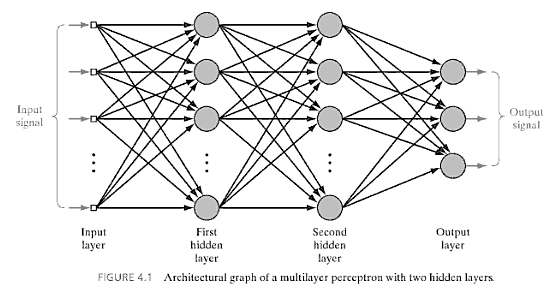
\includegraphics[scale=0.5]{mlp_structure.png}
\caption{MLP Neural Net structure}
\end{figure} 
\end{frame} 

\begin{frame}
\frametitle{MLP Neuron}
\begin{figure}
\centering
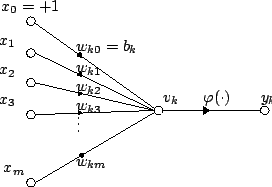
\includegraphics[scale=0.5]{neuron.png}
\caption{MLP neuron}
\end{figure} 
\end{frame}

\begin{frame}
\frametitle{MLP Neuron}
\begin{figure}
\centering
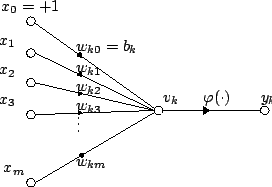
\includegraphics[scale=0.5]{neuron.png}
\caption{MLP neuron}
\end{figure} 
\end{frame}

\begin{frame}[fragile]
\frametitle{Training the Net}
\begin{verbatim}
For each layer
  do the feedforward step
end for each
  calculate the error
For each layer
  do the backpropagation step
  update the weights
end for each
\end{verbatim}
\end{frame}

\begin{frame}
\frametitle{Matrix representation of the weights}
Inputs:
\[ \left( \begin{array}{ccccc}
i_{0} & i_{1} & i_{2} & ... & i_{N} \end{array} \right)\] 
Weights:
\[ \left( \begin{array}{ccccc}
W_{00} & W_{01} & W_{02} & ... & W_{0M} \\
W_{10} & W_{11} & W_{12} & ... & W_{1M} \\
... & ... & ... & ... & ... \\
W_{N0} & W_{N1} & W_{N2} & ... & W_{NM} \end{array} \right)\] 

Where: \\
N - number of inputs \\
M - number of neurons in the layer \\
Note: \\
The output can be calculated by applying the activation function to this product: \\
\[O = I * W\]

\end{frame}

\begin{frame}[fragile]
\frametitle{Backpropagation using gradient descent}
\begin{verbatim}
//for the last layer
auto delta = d_targetVals[i] - d_activationResults[i];
	d_gradients[i] = delta * 
	cuda_activeationFuncD(d_activationResults[i]);

//for hidden layers
d_gradients[i] = d_deltas[i] * 
	cuda_activeationFuncD(d_activationResults[i]);
\end{verbatim}
\end{frame}

\begin{frame}[fragile]
\frametitle{Calculating the deltas for the hidden layer}
\begin{verbatim}
for (auto i = 0; i < static_cast<decltype(i)>(sizeGrad); ++i)
{
   d_deltas[threadId] += d_weights[i * sizeOutput
   + threadId] * d_gradients[i];
}
\end{verbatim}
\end{frame}

\begin{frame}[fragile]
\frametitle{Updating the weights}
\begin{verbatim}
auto deltaWeight = trainRate * d_activationResults[idx] 
   * d_gradients[idx] + momentum * oldDeltaWeight;
d_weights[i] += d_deltaWeights[i];
\end{verbatim}
\end{frame}

\begin{frame}
\frametitle{Normalizing the weights after update}
\begin{itemize}
\item Problem: the activation functions usually accept values between 0.0 and 0.1 (ex: sigmoid) or -1.0 and 1.0 ( ex: hyperbolic tangent). 
\item Solution: the weights need to be normalized to be inside these intervals.
\item The minimum and maximum values needed for the normalization are calculated using reduction.
\end{itemize}
\end{frame}

\begin{frame}
\frametitle{Implementation of the nerual net (Naive method)}
\begin{itemize}
\item Keep the layers (weights, gradients) in the RAM. 
\item Parallelize key methods by writing cuda kernels.
\item In every iteration send the values to the GPU, do the calculation, copy back the result.
\item Very ineffective solution, the GPU is barely used, a lot of time is wasted by doing memory allocation and copying. 
\end{itemize}
\end{frame}

\begin{frame}
\frametitle{Implementation of the nerual net (Optimized approach)}
\begin{itemize}
\item Keep the layers (weights, gradients) in the GPU memory. Use RAII classes, the GPU memory is freed up when the net is deleted. 
\item Parallelize every method by writing cuda kernels.
\item The weights are initialized at the beginning and they are updated when an iteration is done. The inputs are sent in every iteration to the GPU. 
\end{itemize}
\end{frame}

\begin{frame}
\frametitle{Benchmarks}
\begin{itemize}
\item The goal is to learn a sinus curve (20 points).
\item The layer topology is: (1, 1), (1, 10), (10, 10), (10, 10), (10, 1)
\item Avarage time using CPU: 13 milliseconds \ iteration
\item Avarage time using GPU: 18 milliseconds \ iteration
 
\end{itemize}
\end{frame}

\begin{frame}
\frametitle{References}
\begin{itemize}
\item  David Miller - Neural Net in C++ (https://vimeo.com/19569529)
\item  http://iamtrask.github.io/2015/07/27/python-network-part2/
\item  James A. Freeman - Neural Networks - Algorithms, Applications, and Programming Techniques
\end{itemize}
\vspace{1cm}
\centering
Source code and documentation of this project can be found here: https://github.com/Ernyoke/cuda_NN
\end{frame}

\end{document}